% Mathematical tree regression derived from TikZ missing-child semantics.
\documentclass[border=2pt]{standalone}
\usepackage{tikz}
\usetikzlibrary{trees}

\begin{document}
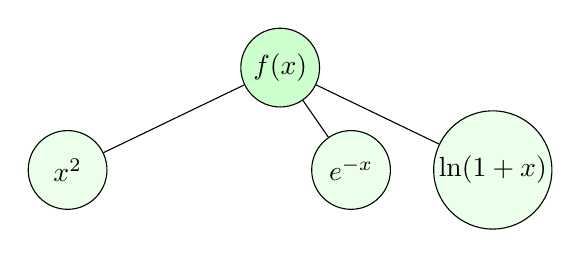
\begin{tikzpicture}[
  grow=down,
  level distance=13mm,
  sibling distance=18mm,
  every node/.style={draw,circle,minimum size=10mm,inner sep=1pt,fill=green!8}
]
  \node[fill=green!20] {$f(x)$}
    child {node {$x^2$}}
    child[missing] {node {$\sin x$}}
    child {node {$e^{-x}$}}
    child[missing=false] {node {$\ln(1+x)$}};
\end{tikzpicture}
\end{document}
